\chapter{Monster black holes in compact massive spheroids with intermediate scale discs}
\label{ch:ellic}

This Chapter brings together three ``hot topics'' of today's astrophysical debate, 
that is, over-massive black holes in the $M_{\rm BH} - L_{\rm sph}$ diagram, 
the variety of intrisic angular momentum radial profiles in local early-type galaxies, 
and the evolution of the mass-size relationship from $z=2$ to $z=0$. 
While an overview about the $M_{\rm BH} - L_{\rm sph}$ outliers was given in Section \ref{sec:monsters}, 
the second topic was only briefly touched in Section \ref{sec:photokin}, 
and no mention of the mass-size relation was made in Chapter \ref{ch:intro} 
because not immediately related to SMBHs. 
Therefore, a more extensive introduction for these last two points is given here. \\ 

\citet{daddi2005} reported on the observation of seven quiescent early-type galaxies 
at $z=1.4-2.5$ with stellar masses $\gtrsim 10^{11} \rm~M_\odot$ 
and effective radii significantly smaller than those of local couterparts. 
\citet{trujillo2006} analysed ten massive $\approx 5 \times 10^{11} \rm~M_\odot$ galaxies at $z=1.2-1.7$ 
and measured for them sizes a factor of 4 smaller than $z=0$ galaxies with similar stellar masses. 
From this, they concluded that the observed rapid evolution of the structural properties of massive quiescent galaxies 
over the last $\approx 10 \rm~Gyr$ 
cannot be reconciled with a monolithic formation scenario. 
\citet{kriek2008} and \citet{vandokkum2008} found that nearly half of $z \approx 2$ 
massive ($\approx 10^{11} \rm~M_\odot$) galaxies 
have old stellar populations, negligible star formation, and sizes a factor of 5 smaller than 
those of the local descendants. 
 
progenitor bias
intermediate scale disc galaxies (arnold)

compact massive spheroids

n1277 paper


The remainder of this chapter comprises the published version of the paper 
``Explaining the reportedly overmassive black holes in early-type galaxies with intermediate-scale discs'' 
by G.~A.~D.~Savorgnan \& A.~W.~Graham,  
as it appears in Volume 457 of \emph{Monthly Notices of the Royal Astronomical Society}. 

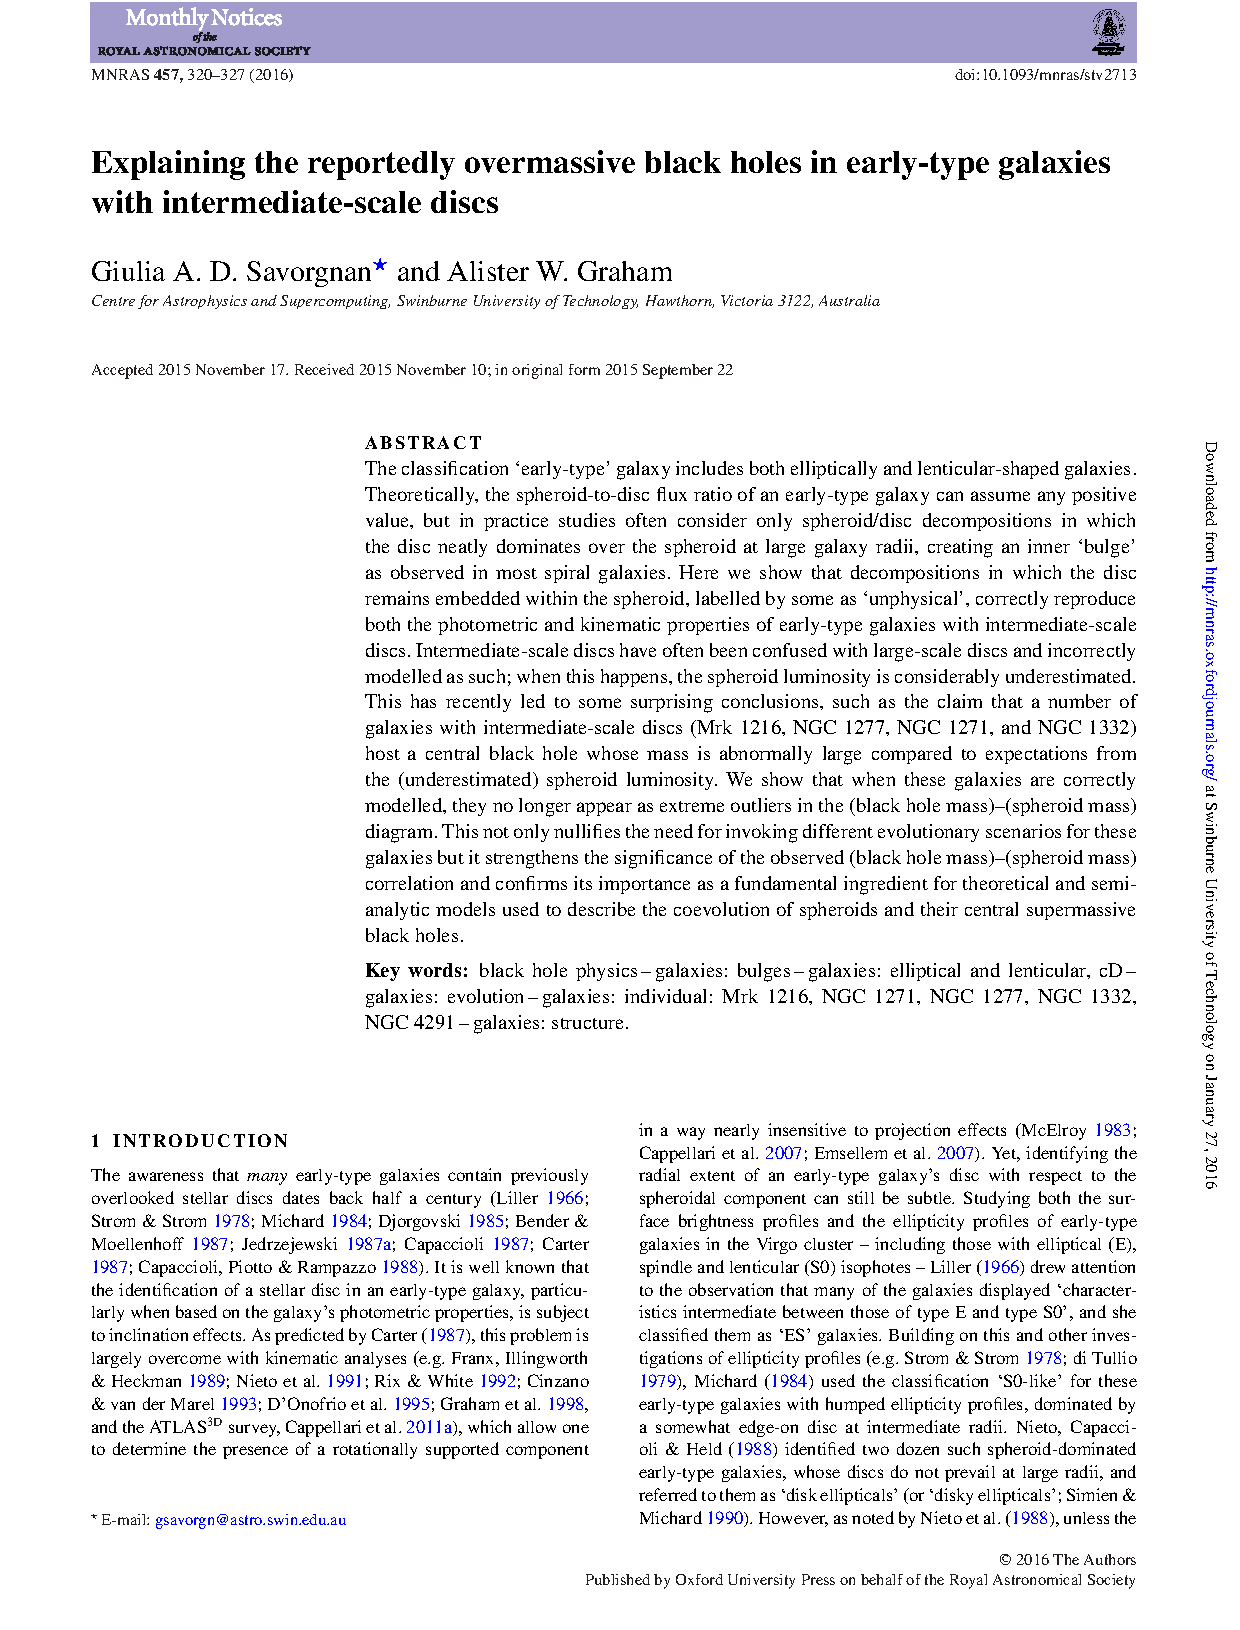
\includepdf[pages={1-8}]{MNRAS2016.pdf}
